\documentclass{UnBeamer}%
%\documentclass[draft]{UnBeamer	}%
% \documentclass[handout]{UnBeamer}%
% \documentclass[notasDeAula]{UnBeamer}%

\usepackage{../ED}%
\usepackage{ED_Grafo}%
% \usepackage{gnramos}%
% \usepackage{electComp}%
% \usepackage{calc}%

% \includeonlyframes{notas}%

\title{Grafos}
\subtitle{Estruturas de Dados Não-lineares}%

\begin{document}%
    \frame[label=notas]{\titlepage}%
    \section{\inserttitle}%
	%!TEX root = ED_Grafo.tex

\section{Conceito}
\begin{frame}[label=notas]
	Grafo: uma representação de relações (arestas) entre objetos (vértices).
	\vfill\pause
	Um grafo $G=(V,A)$ é definido por:
	\begin{description}
		\item[$V$] conjunto de vértices (nós).
		\item[$A$] conjunto de arestas (arcos), que são pares [ordenados] de 
		vértices de $V$.
	\end{description}
	\vfill\pause
	Exemplo:
	\begin{itemize}
		\item[V] = \{A,B,C,D,E,F\}
		\item<4->[A] = \{(A,B), (B,C), (B,D), (D,A), (D,C), (E,F)\}
	\end{itemize}
	\vfill\pause
	\begin{center}
		\begin{tikzpicture}
			\drawABCDnodes%
			\drawEFnodes%
			\pause%
			\drawABCDedges%
			\drawEFedges%
		\end{tikzpicture}
	\end{center}
\end{frame}

\begin{frame}
	\framesubtitle{Aplicações}
	
	\pause
	\begin{itemize}
		\item[$G=$] (Cidades, Estradas)
		\item[$G=$] (Dispositivos Eletrônicos, Conexões)
		\item[$G=$] (Tarefas, Dependências)
		\item[$G=$] (Pessoas, Parentesco)
		\item[$G=$] (etc., etc.)
	\end{itemize}
\end{frame}%
	%!TEX root = ED_Grafo.tex

\section{Definições}
	\begin{frame}[label=notas]
		\framesubtitle{Variações de grafos}
		\begin{columns}
			\column{.475\textwidth}
				\begin{tikzpicture}%
					\node[draw, circle]	(A)		  {A};
					\node[draw, circle]	(B) at(30:2)  {B} edge[line] (A);
					\node[draw, circle]	(C) at(-30:2) {C};
					\draw<1-5>[line]   		(C) -- (A);
					\node<2->          					at(50:1)  {0.75};
					\node<2-5>         					at(-50:1) {2};
					\draw<3-5>[line]       	(C) -- (B);
					\node<3-5>             	           				at(0:1.5) {1};
					\draw<4->[line] (B)..controls +(south east:1) and +(north east:1) .. (C);
					\draw<4->[line] (B)..controls +(north west:1.5) and +(north east:1.5) .. (B);
					\node<4->             	           				at(0:2.8) {1000};
					\node<4->             	           				at(33:3.1) {3.14};
					\node<5->[draw, circle]	(D) at(10:4)	  {D};
				\end{tikzpicture}%
				\begin{itemize}
					\item Não-orientado
					\item<2-> Ponderado % cada aresta tem um peso associado.
					\item<3-> Cíclico % possui caminho de um vértice a ele mesmo
					\item<4-> Multigrafo % existe um vértice com um laço ou um par de vértices conectados por mais de uma aresta
					\item<5-> Desconexo % existe pelo menos um par de vértices enrte os quais não há um caminho
					\item<6-> Parcial % contém todos os nós de $G$ mas apenas um subconjunto de seus arcos.
				\end{itemize}
			\column{.475\textwidth}
				\begin{tikzpicture}%
					\node<1-5>[draw, circle] (A)	  {A};
					\node[draw, circle] (B) at(30:2)  {B};
					\node[draw, circle] (C) at(-30:2) {C} edge[<-,line] (B);
					\draw<1-5>[<-, line] (B) -- (A);
					\draw<3-5>[->,line] (A) -- (C);
					\draw<4->[->,white] (B)..controls +(north west:1.5) and +(north east:1.5) .. (B);
					\node<6->[circle,white] (A) {A};
				\end{tikzpicture}%
				\begin{itemize}[<+->]
					\item Orientado
					\item<2-> Não-ponderado
					\item<3-> Acíclico % não possui circuito.
					\item<4-> Simples %
					\item<5-> {[Fracamente] Conexo} % Existe um caminho entre um par qualquer de vértices (u,v) de modo que u é alcançavel de v mas não o contrário
					\item<6-> Subgrafo % grafo cujo conjunto de vértices é um subconjunto do conjunto de vértices $G$ e o conjunto de arestas é um subconjunto do conjunto de arestas de $G$.
				\end{itemize}
		\end{columns}
	\end{frame}

\begin{frame}[label=notas]
	\begin{description}[<+->]%
		\item[Incidência]\ % uma aresta incidente é o que chega ao vértice. 
		\item[Adjacência]\ % vértices adjacentes estão ligados por uma aresta, arestas adjacentes incidem sobre o mesmo vértice 
		\item[Grau] {[de entrada/saída]} do vértice% número de arestas incidentes em $v$.
		\vfill
		\item[Caminho]\ % sequência de arcos levando de um vértice a outro.
		\item[Alcançável]\ % um vértice $x$ é alcançável a partir do vértice $y$ se existe um caminho de $y$ até $x$.
		\item[Circuito/Laço]\ %circuito é um caminho que leva de um vértice a ele mesmo sem repetições (de vértices), laço é um ciclo formado por uma aresta
	\end{description}
\end{frame}%
	%!TEX root = ED_Grafo.tex

\section{Implementação}
% \begin{frame}[label=notas]
% 	\framesubtitle{Matriz de Adjacência}
	
% 	\begin{itemize}
% 		\item Cada posição na matriz é um arco:
% 			\begin{itemize}
% 				\item linha indica o nó de saída do arco
% 				\item coluna indica o nó de chegada
% 			\end{itemize}
% 		\pause
% 		\item Valor da posição indica:
% 			\begin{itemize}
% 				\item a existência ou não do arco
% 				\item o peso associado ao arco
% 			\end{itemize}
% 		\pause
% 		\item Deve ser utilizada para grafos densos, onde o número de arcos $|A|$ 
% 		é próximo do número de vértices ao quadrado $|V|^2$
% 		\subitem{Complexidade de espaço $O(V^2)$}
% 		\item O tempo necessário para acessar um elemento é  constante.
% 		\item Ler ou examinar  a matriz tem complexidade de 
% tempo $O(V^2)$
% 	\end{itemize}
% \end{frame}

\begin{frame}[label=notas]
	\framesubtitle{Matriz de Adjacência}

	\begin{columns}[T]
     	\column{.5\textwidth}\centering
     		
\includegraphics[width=.8\textwidth]{graph_matrix1}
     	\pause
     	\column{.5\textwidth}\centering
     		
\includegraphics[width=.8\textwidth]{graph_matrix2}
	\end{columns}
\end{frame}

% \begin{frame}[fragile,label=notas]
%	\framesubtitle{Lista de Adjacência}
 	
%	\begin{itemize}
%		\item Os vértices de uma lista de adjacência são em geral armazenados em 
%		uma ordem arbitrária.
%		\item Possui uma complexidade de espaço $O(|V|+|A|)$
%		\item Indicada para grafos esparsos, onde $|A|$ é muito menor do que $|V|^2$ .
%		\item é compacta e usualmente utilizada na maioria das aplicações.
%		\item Tempo $O(|V|)$ para determinar se existe uma aresta entre 
%		o vértice $i$ e o vértice $j$, pois podem existir $O(|V|)$vértices na 
%		lista de adjacentes do vértice $i$.
%	\end{itemize}
%	\begin{center}
%	\begin{minipage}{.35\textwidth}
%	\begin{lstlisting}[title=Vértice]
% typedef struct v_node_t {
%     char cidade[20];
%     a_node_t *aresta;
%     struct v_node_t *prox;
% } v_node_t;
%	\end{lstlisting}
%	\end{minipage}
%	\hspace{1cm}
%	\begin{minipage}{.4\textwidth}
%	\begin{lstlisting}[title=Aresta]
% typedef struct a_node_t {
%     double peso;
%     struct v_node_t *vertice;
%     struct a_node_t *prox;
% } a_node_t;
%	\end{lstlisting}
%	\end{minipage}
%	\end{center}
% \end{frame}

\makeatletter%
\newcommand{\vertice}[2][\@empty]{%
	\ifx#1\@empty%
		\node[block, fill=greenUnB, minimum size=2em] (#2) {\textcolor{white}{\large\textbf{#2}}};
	\else%
		\node[block, fill=greenUnB, minimum size=2em, below of=#1] (#2) {\textcolor{white}{\large\textbf{#2}}} edge[line, greenUnB, <-] (#1);
	\fi%
}%
\makeatother%
\newcommand{\aresta}[3]{%
	\node[block, blueUnB, minimum size=2em, right of=#1] (#1#2) {$#3 \overrightarrow{#2}$} edge[line,blueUnB,<-] (#1);
}%
\begin{frame}[label=notas]
	\framesubtitle{Lista de Adjacência}
	
	\begin{tikzpicture}[scale=1.5]
		\drawABCDnodes
		\drawABCDdirectedEdges
		\drawABCDweights
	\end{tikzpicture}
	\hfill\pause
	\begin{tikzpicture}[node distance=15mm]
		\vertice{A}
		\vertice[A]{B}
		\vertice[B]{C}
		\vertice[C]{D}
		
		\pause
		\aresta{A}{B}{0.3}
		\draw<3>[->, dashed] (AB)..controls +(south east:0.5) and +(north east:1) .. (B);
		\pause
		\aresta{B}{A}{0.4}
		\aresta{BA}{C}{0.2}
		\aresta{BAC}{D}{0.7}
		\draw<4>[->, dashed] (BA)..controls +(north east:0.5) and +(south east:1) .. (A);
		\draw<4>[->, dashed] (BAC)..controls +(south east:0.5) and +(north east:1) .. (C);
		\draw<4>[->, dashed] (BACD)..controls +(south east:0.5) and +(north east:1) .. (D);
		
		\pause
		\aresta{C}{C}{0.5}
		\aresta{CC}{D}{0.1}
		\aresta{D}{A}{0.8}
		\aresta{DA}{C}{1}
	\end{tikzpicture}
\end{frame}%
	%!TEX root = ED_Grafo.tex

\section{Travessia / Busca}
\begin{frame}[label=notas]
	\framesubtitle{Travessia/Percurso/Transversalização}

	Travessia: percorrer cada elemento ``uma'' vez.
	\\\vfill\pause
	Algoritmo Simples:\pause
	\begin{enumerate}
		\item Enquanto o conjunto $V$ de vértices não visitados não for vazio:
			\begin{enumerate}
				\item Retire um vértice $u$ de $V$.
				\item Processe o $u$.
				\item Insira $u$ no conjunto de vértices visitados $V'$
			\end{enumerate}
	\end{enumerate}
	% \begin{center}
 %  	\begin{minipage}{.8\textwidth}
%   	\begin{lstlisting}[morekeywords={travessia_em_grafos,estado_inicial,vazia,retira_um,objetivo,expande, e}]
% travessia_em_grafos(problema)
%     a_visitar:=  estado_inicial(problema)
%     nos_visitados:=  emptyset
%     enquanto(verdadeiro)
%         se(a_visitar= emptyset) retorna FALHA
%         folha:= retira_um(a_visitar)
%         se(folha = objetivo(problema)) retorna SUCESSO
%         nos_visitados += folha
%         para_cada(no pertence  expande(folha))
%             se(no nao_pertence a_visitar e no nao_pertence nos_visitados)
%                 a_visitar += no
% \end{lstlisting}
		% \end{minipage}
		% \end{center}
\end{frame}

\begin{frame}[label=notas]
	Busca:\pause\ \textbf{s. f.} 1. Ato de buscar. 2. Pesquisa.
	\\\vfill\pause
	Busca em uma estrutura de dados\alt<1-3>{?}{ é a aplicação de um algoritmo
	para encontrar um item específico em um conjunto de items (registros distintos,
	elementos de um domínio definido por uma função matemática, ou uma combinação
	de ambos).}\pause
	\\\vfill
	Algoritmo Simples:\pause
	\begin{enumerate}
		\item Enquanto o conjunto não for vazio:
			\begin{enumerate}
				\item \alert<6>{Escolha} um item do conjunto
				\item Se o item for o desejado, termine.
				\item Senão, retire-o do conjunto.
			\end{enumerate}
	\end{enumerate}
\end{frame}

\begin{frame}
	\framesubtitle{Busca em Profundidade}
	A estratégia é \alert{escolher o vértice mais profundo} para avaliação.
	\vfill
	\begin{center}
		\includegraphics<1 | handout:0>{dfs-progress01c}
		\includegraphics<2 | handout:0>{dfs-progress02c}
		\includegraphics<3 | handout:0>{dfs-progress03c}
		\includegraphics<4 | handout:0>{dfs-progress04c}
		\includegraphics<5 | handout:0>{dfs-progress05c}
		\includegraphics<6 | handout:0>{dfs-progress06c}
		\includegraphics<7 | handout:0>{dfs-progress07c}
		\includegraphics<8 | handout:0>{dfs-progress08c}
		\includegraphics<9 | handout:0>{dfs-progress09c}
		\includegraphics<10 | handout:0>{dfs-progress10c}
		\includegraphics<11 | handout:0>{dfs-progress11c}
		\includegraphics<12>{dfs-progress12c}
	\end{center}
\end{frame}

\begin{frame}
	\framesubtitle{Busca em Largura (em Extensão)}

	\begin{itemize}
		\item A estratégia é \alert{escolher o vértice mais raso} para avaliação.
		\item O algoritmo descobre todos os vértices a uma distância $k$ do vértice 
		origem antes de descobrir qualquer vértice a uma distância $k + 1$.
	\end{itemize}
	\vfill
	\begin{center}
		\includegraphics<1 | handout:0>{bfs-progress1c}
		\includegraphics<2 | handout:0>{bfs-progress2c}
		\includegraphics<3 | handout:0>{bfs-progress3c}
		\includegraphics<4 | handout:0>{bfs-progress4c}
	\end{center}
\end{frame}


% \begin{frame}[fragile,label=notas]
% 	\framesubtitle{Busca em Profundidade - Algoritmo}
	
% 	Enquanto a pilha não está vazia faça:
% 	\begin{enumerate}
% 		\item Seja  $v$  o vértice no topo da pilha e $A_V$ seus arcos.
% 		\item Se $A_V \neq \emptyset$, então retire uma aresta $(v,w)$ de $A_V$:
% 			\begin{itemize}
% 				\item Se $w$ não está marcado
% 				\begin{enumerate}[(i)]
% 					\item Então então marque $w$
% 					\item Coloque $w$ na lista de arcos visitados
% 				\end{enumerate} 
% 			\end{itemize} 
% 		\item Senão, retire $v$ do topo da pilha.
% 	\end{enumerate}
% \end{frame}


% \begin{frame}[label=notas]
% 	\framesubtitle{Busca em Largura (em Extensão) - Algoritmo}

% 	\begin{enumerate}
% 		\item Coloca o nó raiz na fila.
% 		\item Retira um nó do início da fila e o examina.
% 		\item Se o elemento procurado está nesse nó, interrompe a busca e retorna 
% 		o resultado.
% 		\item Senão, coloca todos os sucessores desse nó, ainda não 
% examinados, no final da lista. 
% 		\item Se a fila está vazia, cada nó no grafo já foi examinado
% 			\subitem{interrompe a busca e retorna ``não encontrado''.}
% 		\item Repete passo 2.
% 	\end{enumerate}
% \end{frame}

\begin{frame}
	\framesubtitle{Análise de Complexidade}
	
	\begin{itemize}[<+->]
		\item Estruturas de dados adequadas para cada busca?
		\item Complexidade temporal de ambos os algoritmos de busca é $O(|V|{\cdot}|A|)$.
		\vfill
		\item Complexidade espacial da busca em profundidade é $O(h)$, onde $h$ 
		é o comprimento do caminho mais longo no grafo.
		\item Complexidade espacial da busca em largura é $O(|V|{\cdot}|A|)$
	\end{itemize}
\end{frame}

\begin{frame}
	\framesubtitle{Busca Profundidade $x$ Largura}
	
	\begin{itemize}
		\item A busca em largura é completa apenas se nenhum vértice tem grau infinito\pause, a em profundidade se não houver um caminho de comprimento infinito.\vfill
		\item A busca em largura é ótima se o custo dos passos forem  idênticos.
		\pause\vfill
		\item A busca em profundidade é aplicada em vários algoritmos de ordenação 
		em grafos como:
		\begin{itemize}
	\item Ordenamento topológico.
	\item Encontrar componentes fortemente conectados.
		\end{itemize}
	\end{itemize}
\end{frame}

\newcommand{\sfrac}[2]{$^{#1}/_{#2}$}%
\newcommand{\canoaEsq}[2]{\sfrac{c#1}{#2}}%
\newcommand{\canoaDir}[2]{\sfrac{#1}{#2c}}%
\begin{frame}
	\framesubtitle{Exemplo de Aplicação: Missionários e Canibais}

	3 missionários e 3 canibais estão em um lado de um rio, e há uma canoa onde 
	cabem até 2 pessoas. Como levar todos ao outro lado do rio sem que, havendo 
	pelo menos um missionário na margem, não haja mais canibais que missionários 
	nela?
	\\\vfill\pause
	Supondo a representação: \LARGE \canoaEsq{MargemEsquerda}{MargemDireita}
\end{frame}

\newcommand{\ellipse}[2][blue]{%
	\draw[line width=1pt,#1] (#2) ellipse [x radius=1cm,y radius=.5cm];
}

\begin{frame}[label=notas]
	\framesubtitle{Exemplo: Missionários e Canibais}

	\Large
	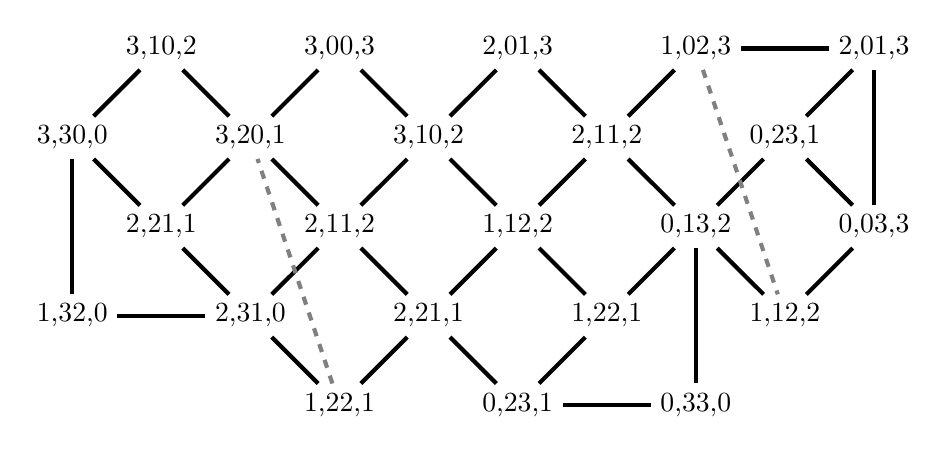
\begin{tikzpicture}[node distance=16mm]%[every node/.style={circle,draw},node distance=2cm]
		\node (c3300) {\canoaEsq{3,3}{0,0}};
		\pause
		%\node[above left of=c3300] (2310c) {\canoaDir{2,3}{1,0}} edge[line width=1.5pt] (c3300);
		%\node[below left of=c3300] (2301c) {\canoaDir{3,2}{0,1}} edge[line width=1.5pt] (c3300);
		\node[above right of=c3300] (3102c) {\canoaDir{3,1}{0,2}} edge[line width=1.5pt] (c3300);
		\node[below right of=c3300] (2211c) {\canoaDir{2,2}{1,1}} edge[line width=1.5pt] (c3300);
		\node[below left of=2211c] (1320c) {\canoaDir{1,3}{2,0}} edge[line width=1.5pt] (c3300);
		\pause
		\node[below right of=3102c] (c3201) {\canoaEsq{3,2}{0,1}} edge[line width=1.5pt] (3102c);
		\draw[line width=1.5pt] (c3201) -- (2211c);
		\node[below right of=2211c] (c2310) {\canoaEsq{2,3}{1,0}} edge[line width=1.5pt] (2211c);
		\draw[line width=1.5pt] (c2310) -- (1320c);
		\pause
		\node[above right of=c3201] (3003c) {\canoaDir{3,0}{0,3}} edge[line width=1.5pt] (c3201);
		\node[below right of=c3201] (2112c) {\canoaDir{2,1}{1,2}} edge[line width=1.5pt] (c3201);
		\draw[line width=1.5pt] (2112c) -- (c2310);
		\node[below right of=c2310] (1221c) {\canoaDir{1,2}{2,1}} edge[line width=1.5pt] (c2310);
		\draw[line width=1.5pt,dashed,gray] (1221c) -- (c3201);
		\pause
		\node[above right of=2112c] (c3102) {\canoaEsq{3,1}{0,2}} edge[line width=1.5pt] (2112c);
		\draw[line width=1.5pt] (3003c) -- (c3102);
		\node[above right of=1221c] (c2211) {\canoaEsq{2,2}{1,1}} edge[line width=1.5pt] (2112c);
		\draw[line width=1.5pt] (1221c) -- (c2211);
		\pause
		\node[above right of=c2211] (1122c) {\canoaDir{1,1}{2,2}} edge[line width=1.5pt] (c2211);
		\draw[line width=1.5pt] (1122c) -- (c3102);
		\node[above right of=c3102] (2013c) {\canoaDir{2,0}{1,3}} edge[line width=1.5pt] (c3102);
		\node[below right of=c2211] (0231c) {\canoaDir{0,2}{3,1}} edge[line width=1.5pt] (c2211);
		\pause
		\node[below right of=2013c] (c2112) {\canoaEsq{2,1}{1,2}} edge[line width=1.5pt] (2013c);
		\draw[line width=1.5pt] (c2112) -- (1122c);
		\node[below right of=1122c] (c1221) {\canoaEsq{1,2}{2,1}} edge[line width=1.5pt] (1122c);
		\draw[line width=1.5pt] (c1221) -- (0231c);
		\node[below right of=c1221] (c0330) {\canoaEsq{0,3}{3,0}} edge[line width=1.5pt] (0231c);
		\pause
		\node[above right of=c2112] (1023c) {\canoaDir{1,0}{2,3}} edge[line width=1.5pt] (c2112);
		\node[above right of=c1221] (0132c) {\canoaDir{0,1}{3,2}} edge[line width=1.5pt] (c1221);
		\draw[line width=1.5pt] (c2112) -- (0132c);
		\draw[line width=1.5pt] (c0330) -- (0132c);
		\pause
		\node[below right of=1023c] (c0231) {\canoaEsq{0,2}{3,1}} edge[line width=1.5pt] (0132c);
		\node[below right of=0132c] (c1122) {\canoaEsq{1,1}{2,2}} edge[line width=1.5pt] (0132c);
		\draw[line width=1.5pt,dashed,gray] (1023c) -- (c1122);
		\pause
		\node[below right of=c0231] (0033c) {\canoaDir{0,0}{3,3}} edge[line width=1.5pt] (c0231);
		\draw[line width=1.5pt] (0033c) -- (c1122);
		\node[above right of=c0231] (c2013) {\canoaEsq{2,0}{1,3}} edge[line width=1.5pt] (c0231);
		\draw[line width=1.5pt] (0033c) -- (c2013);
		\draw[line width=1.5pt] (1023c) -- (c2013);
		\pause
		\ellipse{c3300}
		\pause
		\ellipse{2211c}
		\ellipse{3102c}
		\ellipse[red]{1320c}
		\pause
		\ellipse{c3201}
		\ellipse[red]{c2310}
		\pause
		\ellipse{3003c}
		\ellipse[red]{2112c}
		\ellipse[red]{1221c}
		\pause
		\ellipse{c3102}
		\pause
		\ellipse{1122c}
		\ellipse[red]{2013c}
		\pause
		\ellipse[red]{c2112}
		\ellipse{c2211}
		\ellipse[red]{c1221}
		\pause
		\ellipse{0231c}
		\pause
		\ellipse{c0330}
		\pause
		\ellipse[red]{1023c}
		\ellipse[red]{c2013}
		\ellipse{0132c}
		\ellipse{c0231}
		\ellipse{c1122}
		\ellipse[green,line width=2pt]{0033c}
	\end{tikzpicture}
\end{frame}

\begin{frame}
	\framesubtitle{Exemplo: Missionários e Canibais}

	Supondo que só se explore nós que não violam as restrições e a representação $MCK$, onde:
	\begin{itemize}
		\item[M] número de missionários \emph{na margem errada}.
		\item[C] número de canibais \emph{na margem errada}.
		\item[K] número de canoas \emph{na margem errada}.
	\end{itemize}

	\vfill
	\begin{center}
		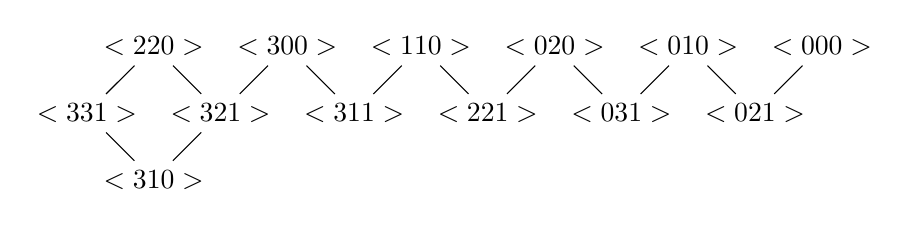
\begin{tikzpicture}[node distance=12mm]%
			\node (331){$<331>$};
			\pause
			\node[above right of=331] (220){$<220>$} edge (331);
			\node[below right of=331] (310){$<310>$} edge (331);
			\pause
			\node[below right of=220] (321){$<321>$} edge (220) edge (310);
			\pause
			\node[above right of=321] (300){$<300>$} edge (321);
			\node[below right of=300] (311){$<311>$} edge (300);
			\node[above right of=311] (110){$<110>$} edge (311);
			\node[below right of=110] (221){$<221>$} edge (110);
			\node[above right of=221] (020){$<020>$} edge (221);
			\node[below right of=020] (031){$<031>$} edge (020);
			\node[above right of=031] (010){$<010>$} edge (031);
			\node[below right of=010] (021){$<021>$} edge (010);
			\node[above right of=021] (000){$<000>$} edge (021);
		\end{tikzpicture}
	\end{center}
\end{frame}

\begin{frame}
	\framesubtitle{\url{http://www.youtube.com/watch?v=DINCL5cd_w0}}
	\begin{center}
		\href{run:vid/Pathfinding.mp4}{
\includegraphics[width=\textwidth]{dijkstra.png}}
	\end{center}
\end{frame}%
	%!TEX root = ED_Grafo.tex

\section{Exemplos}
\begin{frame}
	\frametitle{Exercício}
	\framesubtitle{Algoritmo para Encontrar Amigos em uma Rede Social}
	
	Dada uma rede social representada por um grafo, onde cada aresta representa 
	uma relação de amizade, elabore um algoritmo que liste sugestões de prováveis 
	amigos. \pause Uma pessoa pode ser sugerida a outra se elas não são amigas 
	(na rede social) e têm pelo menos $n$ amigos em comum.
	\pause
	\begin{enumerate}
		\item Suponha o grafo $G(V,A)$ e um vértice $v$ inicial.
		\item Para cada vértice $u$ tal que $^{\exists}(v,u)$:
			\begin{enumerate}
				\item Para cada vértice $w \not\in\{v,u\}$ tal que $^{\exists}(u,w)$:
				\subitem[]{Se $\not\exists (v,w)$: incremente $contador\_W$.}
				\item Se $contador\_W \geq n$: adicione $w$ a lista de sugestões.
			\end{enumerate}
		\item Retorne a lista de sugestões.
	\end{enumerate}
\end{frame}

\begin{frame}[label=notas]
	\frametitle{Exercício}
	\framesubtitle{Encontrar Amigos de $A$}
	
	\begin{center}
		\begin{tikzpicture}[every node/.style={circle,draw},node distance=15mm]
			\node (A) {A};
			\node[above right of=A] (B) {B} edge (A);
			\node[below right of=A] (C) {C} edge (A);
			\node[right of=A] (D) {D} edge (A) edge (B) edge (C);
			\node[right of=D] (E) {E} edge (B) edge (C) edge (D);
			\node[left of=A] (K) {K} edge (A);
			\node[below of=K] (F) {F} edge (A) edge (C);
			\node[above left of=K] (G) {G} edge (B) edge (F);
			\node[above right of=G] (H) {H} edge (B) edge (G);
			\node[above of=B] (I) {I} edge (B) edge (H);
			\node[above of=E] (J) {J} edge (B) edge (E) edge (I);
			\node[above right of=J, right = 2\baselineskip, label=right:{L}] (L) {
\includegraphics[width=.1\textwidth]{foreveralone}};
		\end{tikzpicture}
		\\\vfill		
		\uncover<2->{
		\begin{tabular}{*{13}{|c}|}
			\hline
			& A & B & C & D & E & F & G & H & I & J & K & L\\\hline
			contador & 0 & 0 & 0 & 0 & 3 & 0 & 2 & 1 & 1 & 1 & 0 & 0 \\\hline
		\end{tabular}
		}
	\end{center}
	\begin{columns}[T]
		\column{.45\textwidth}
		\subitem[a)]{Para $n = 3$ \pause $\rightarrow\{E\}$}
		\column{.45\textwidth}
		\subitem[b)]{Para $n = 2$ \pause $\rightarrow\{E, G\}$}
	\end{columns}
\end{frame}

\begin{frame}[label=notas]
	\frametitle{Exemplo: Mapas de Música}
	\framesubtitle{\url{http://audiomap.tuneglue.net/}}
	
	\vfill
	\begin{center}
		
\includegraphics[width=.8\textwidth]{musicmap}
		\framezoom<2 | handout:0><2 | handout:0>[border](10mm,30mm)(4cm,4cm)
	\end{center}
\end{frame}%
	%!TEX root = ED_Grafo.tex

\section{Ordenamento Topológico}
\begin{frame}
	\begin{itemize}
		\item Ordenação linear de todos os vértices, tal que se $G$ contém uma 
		aresta $(u, v)$ então $u$ aparece antes de $v$.
		\item Pode ser vista como uma ordenação de seus vértices ao longo de uma 
		linha horizontal de tal forma que todas as arestas estão direcionadas da 
		esquerda para a direita.
		\item Pode ser usado sempre que o problema abordado envolve uma ordem parcial.
		\item Um grafo pode ter vários ordenamentos topológicos possíveis.
	\end{itemize}
\end{frame}

\begin{frame}[label=notas]
	\begin{columns}[T]
		\column{.5\textwidth}
			\begin{tikzpicture}[every node/.style={circle,draw},node distance=15mm]
				\node (7) {7};
				\node[below right of=7] (11) {11} edge[line,<-] (7);
				\node[above right of=11] (5) {5} edge[line,->] (11);
				\node[below left of=11] (2) {2} edge[line,<-] (11);
				\node[below right of=5] (8) {8} edge[line,<-] (7);
				\node[above right of=8] (3) {3} edge[line,->] (8);
				\node[below left of=8] (9) {9} edge[line,<-] (8) edge[line,<-] (11);
				\node[below right of=8] (10) {10} edge[line,<-] (3) edge[line,<-] (11);
			\end{tikzpicture}
			\pause
		\column{.4\textwidth}
			\begin{enumerate}
				\item 7, 5, 3, 11, 8, 2, 9, 10% (visual esquerda-para-direita, de-cima-para-baixo)
				\item 3, 5, 7, 8, 11, 2, 9, 10 %(vértice de menor número disponível primeiro)
				\item<1- | alert@3-> 3, 7, 8, 5, 11, 10, 2, 9%
				\item 5, 7, 3, 8, 11, 10, 9, 2 %(menor número de arestas primeirofirst)
				\item 7, 5, 11, 3, 10, 8, 9, 2 %(vértice de maior número disponível primeiro)
				\item 7, 5, 11, 2, 3, 8, 9, 10%
			\end{enumerate}
	\end{columns}
	\pause\vfill
	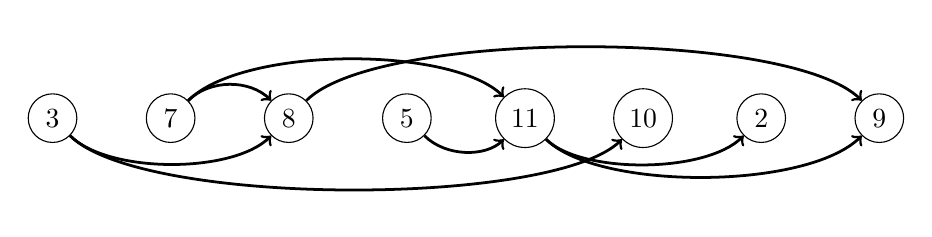
\begin{tikzpicture}[every node/.style={circle,draw},node distance=15mm]
		\node (3) {3};
		\foreach \x/\y in {7/3,8/7,5/8,11/5,10/11,2/10,9/2}
			\node[right of=\y] (\x) {\x};
		\foreach \x/\y/\z in {3/8/1,3/10/1.6,5/11/0.7,11/2/1,11/9/1.3}
			\draw[line width=1pt,->] (\x) ..controls +(south east:\z) and +(south west:\z) .. (\y);
		\foreach \x/\y/\z in {7/11/1.3,7/8/0.7,8/9/1.6}
			\draw[line width=1pt,->] (\x) ..controls +(north east:\z) and +(north west:\z) .. (\y);
	\end{tikzpicture}
\end{frame}

\begin{frame}[fragile]
	Algoritmo para Ordenamento Topológico:
	
	\begin{itemize}
		\item Adaptação da busca em profundidade.
		\item Durante a busca em profundidade, a cada vértice completo, insere na 
		frente de uma lista encadeada.
	\end{itemize}
	
	\begin{center}
		\begin{minipage}{.7\textwidth}
			\begin{lstlisting}[morekeywords={ord_top,v_node_t, processa, vizinho, processado, insere}]
			ordenamento_topologico(G)
				para cada vertice em V
				    g[v] := grau_de_entrada(v)
				    se g[v] = 0
				        insere(fila, v)
				    j := 0
				    enquanto !vazia(fila)
				        v := retira(fila)
				        insere(resultado, v)
				        j := j+1
				        para cada (v,u) em A
				            g[u] := g[u]-1
				            se g[u] = 0
				                insere(fila, v)
			\end{lstlisting}
		\end{minipage}
	\end{center}
\end{frame}

\begin{frame}
	\framesubtitle{Aplicação: Escalonamento}
	
	\pause
	\begin{block}{Escalonamento}
		Organização (distribuição e ordem de execução) de tarefas nos recursos disponíveis.
	\end{block}
	\pause
	Objetivos:
	\begin{itemize}
		\item Ser justo(evitando o adiamento indefinido).
		\item Maximizar a produtividade (\emph{throughput}.
		\item Ser previsível.
		\item Minimizar o tempo de resposta para usuários interativos.
		\item Maximizar o número possível de usuário interativos.
		\item Minimizar a sobrecarga (overhead).
		\item Balancear o uso de recursos.
		\item Exibir degradação previsível e progressiva em situações de intensa 
		carga de trabalho.
		\item Etc.
	\end{itemize}
\end{frame}

\begin{frame}[label=notas]
	\framesubtitle{Aplicação: Escalonamento}
	
	\begin{columns}
		\column{.35\textwidth}
			\begin{enumerate}
				\item Pegar ovo.
				\item Pegar o óleo.
				\item Untar a frigideira.
				\item Quebrar o ovo.
				\item Esquentar o óleo.
				\item Pôr o ovo na frigideira.
				\item Esperar o ovo fritar.
				\item Retirar o ovo.
			\end{enumerate}
		\column{.65\textwidth}
			\pause
			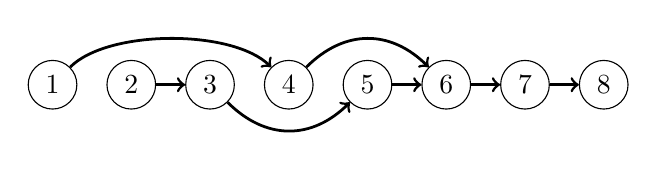
\begin{tikzpicture}[every node/.style={circle,draw}]%,node distance=2cm]
				\node (1) {1};
				\foreach \x/\y in {2/1,3/2,4/3,5/4,6/5,7/6,8/7}
					\node[right of=\y] (\x) {\x};
				\foreach \x/\y in {1/4,4/6}
					\draw[line width=1pt,->] (\x) ..controls +(north east:1) and +(north west:1) .. (\y);
				\foreach \x/\y in {2/3,5/6,6/7,7/8}
					\draw[line width=1pt,->] (\x) -- (\y);
				\draw[line width=1pt,->] (3) ..controls +(south east:1) and +(south west:1) .. (5);
			\end{tikzpicture}\\\vfill\pause
			\begin{tikzpicture}[every node/.style={circle,draw},node distance=13mm]
				\node (1) {1};
				\node[right of=1] (4) {4} edge[line width=1pt,<-] (1);
				\node[below of=4] (5) {5};
				\node[left of=5] (3) {3} edge[line width=1pt,->] (5);
				\node[left of=3] (2) {2} edge[line width=1pt,->] (3);
				\node[right of=4] (6) {6} edge[line width=1pt,<-] (4) edge[line width=1pt,<-] (5);
				\node[right of=6] (7) {7} edge[line width=1pt,<-] (6);
				\node[right of=7] (8) {8} edge[line width=1pt,<-] (7);
				\pause
				\node[rectangle, white, above right of=1] {\textcolor{greenUnB}{Recurso 1}};
				\node[rectangle, white, below of=3, above=3mm] {\textcolor{blueUnB}{Recurso 2}};
				\node[rectangle, white, above of=7, below=3mm] {\textcolor{redUnB}{Recurso ?}};
				\node[rectangle, dashed, line width=2pt, greenUnB, fit=(1) (4)] {};
				\node[rectangle, dashed, line width=2pt, blueUnB, fit=(2) (3) (5)] {};
				\node[rectangle, dashed, line width=2pt, redUnB, fit=(6) (7) (8)] {};
			\end{tikzpicture}
	\end{columns}
\end{frame}

% \begin{frame}
%	\frametitle{Componentes fortemente conectados}

%	Um componente contectado $C$ é o maior conjunto de vértices ${u, v} \in C$ 
%	tal que $u \leadsto v$ e $v \leadsto u$. 

%	\pause \vfill

%	\begin{block}{Aplicabilidade}
%		Uma quantidade significativa de problemas, aparentemente complexos,
%		são reduzidos a identificação ou contagem de componentes
%		fortementes conectados de um grafo.
%	\end{block}
% \end{frame}

% \begin{frame}[label=notas]
%	\frametitle{Exemplo (Fonte: Introduction to Algorithms)}

%	\begin{center}
%	
\includegraphics[scale=0.5]{stronglyConnectedComponents.png}
%	\end{center}
% \end{frame}%
	%!TEX root = ED_Grafo.tex

\section{Aplicações em Inteligência Artificial de Jogos}
\subsection{Grafo de Navegação}
\begin{frame}[label=notas]
	\framesubtitle{Learning AI by Example}
	\begin{columns}
		\column{.5\textwidth}\centering
			
\includegraphics[width=.9\textwidth]{navi_graph}
		\column{.5\textwidth}\centering
			
\includegraphics[width=.9\textwidth]{grid_graph}
	\end{columns}
\end{frame}

\subsection{Grafo de Dependências}
\begin{frame}[label=notas]
	\frametitle{\subsecname\footnote{``Árvore tecnológica''}}
	\framesubtitle{Learning AI by Example}
    \begin{overprint}
		\begin{tikzpicture}[every node/.style={draw,block},every edge/.style={draw,<-,line width=1.5pt}]
			\node              	at(0,0)  	(Prefeitura)	{Prefeitura};
			%\onslide<2->{\node	at(0,-1) 	(Peoes)     	{Peões}     	edge (Prefeitura);
			\onslide<2->{\node 	at(2,0)  	(Mina)      	{Mina}      	edge (Prefeitura);}
			\onslide<2->{\node 	at(0,1)  	(Forte)     	{Forte}     	edge (Prefeitura);}
			\onslide<2->{\node 	at(-2,0) 	(Quartel)   	{Quartel}   	edge (Prefeitura);}
			\onslide<2->{\node 	at(0,-1) 	(Madeireira)	{Madeireira}	edge (Prefeitura);}
			\onslide<3->{\node 	at(-3,1) 	(Cavalaria) 	{Cavalaria} 	edge (Quartel);}
			\onslide<3->{\node 	at(-4,0) 	(Infantaria)	{Infantaria}	edge (Quartel);}
			\onslide<3->{\node 	at(0,-2) 	(Serraria)  	{Serraria}  	edge (Madeireira);}
			\onslide<3->{\node 	at(2,-1) 	(Oficina)   	{Oficina}   	edge (Mina)	edge (Madeireira);}
			\onslide<4->{\node 	at(4,0)  	(Polvora)   	{Pólvora}   	edge (Oficina);}
			\onslide<4->{\node 	at(4,-2) 	(Ferro)     	{Ferro}     	edge (Oficina);}
			\onslide<4->{\node 	at(-2,-2)	(Flechas)   	{Flechas}   	edge (Serraria);}
			\onslide<5>{\node  	at(-3,-1)	(Arqueiros) 	{Arqueiros} 	edge (Quartel)	edge (Flechas);}
			\onslide<5>{\node  	at(0,2)  	(Castelo)   	{Castelo}   	edge (Forte)  	edge (Polvora)	edge (Quartel);}
			\onslide<5>{\node  	at(6,-1) 	(Canhoes)   	{Canhões}   	edge (Ferro)  	edge (Polvora);}
			\onslide<5>{\node  	at(4,-1) 	(Armas)     	{Armas}     	edge (Ferro)  	edge (Polvora);}
		\end{tikzpicture}
    \end{overprint}
\end{frame}

\newcommand{\hanoi}[1]{\includegraphics[scale=0.5]{hanoi_#1}}%
\subsection{Grafo de Estados}
\begin{frame}[label=notas]
	\framesubtitle{Learning AI by Example}
	
    \begin{overprint}
		\begin{tikzpicture}[node distance=2cm,every edge/.style={draw,<->,line width=1.5pt}]
			\node                               	(1)	{\hanoi{2_0_0}};
			\onslide<2->{\node[below right of=1]	(2)	{\hanoi{1_1_0a}}	edge (1);}
			\onslide<2->{\node[above right of=1]	(3)	{\hanoi{1_0_1b}}	edge (1);}

			\onslide<3->{\draw (2)                    	edge (3);}
			\onslide<3->{\node[right of=2, right=-5mm]	(4)	{\hanoi{0_1_1a}}	edge (2);}
			\onslide<3->{\node[right of=3, right=-5mm]	(5)	{\hanoi{0_1_1b}}	edge (3);}

			\onslide<4->{\node[below right of=4]      	(6)	{\hanoi{0_0_2}} 	edge (4);}
			\onslide<4->{\node[right of=4, right=-5mm]	(7)	{\hanoi{1_0_1a}}	edge (4);}
			\onslide<4->{\node[right of=5, right=-5mm]	(8)	{\hanoi{1_1_0b}}	edge (5);}
			\onslide<4->{\node[above right of=5]      	(9)	{\hanoi{0_2_0}} 	edge (5);}
			
			\onslide<5->{\draw (6) edge (7);}
			\onslide<5->{\draw (7) edge (8);}
			\onslide<5->{\draw (8) edge (9);}
		\end{tikzpicture}
    \end{overprint}
\end{frame}%
	%!TEX root = ED_Grafo.tex

\section{Árvore Geradora Mínima}%
\begin{frame}[label=notas]
	Uma árvore geradora é um grafo parcial de $G$ que representa uma árvore.
	\\\vfill\pause
	\begin{block}{Arvore Geradora Mínima}
		Árvore geradora cuja soma dos pesos de todas as arestas é mínima\footnote[frame]{Unicidade?}.
	\end{block}
	\vfill\pause
	Algoritmos:
	\begin{description}
		\item[Genérico:] a cada passo, adiciona-se uma aresta ``segura''
		a um subconjunto de arestas do grafo: o subconjunto final é a AGM.
		\item[Prim:] as arestas adicionadas ao subconjunto (árvore)
		devem ser as de mínimo peso que conectam a árvore a um vértice ainda não presente.
		\item[Kruskal:] as arestas adicionadas as árvores são as arestas
		de menor peso que conectam dois componentes distintos.
	\end{description}
\end{frame}

\begin{frame}
	Outros tipos:
	\begin{description}
		\item[Maximum Spanning Trees] AG com as arestas que resultam no maior
		custo. Implementação?%Suppose we hire an evil telephone company to connect a bunch of houses together, and that this company will be paid a price proportional to the amount of wire they install. Naturally, they will want to build as expensive a spanning tree as possible. The maximum spanning tree of any graph can be found by simply negating the weights of all edges and running Prim’s algorithm. The most negative tree in the negated graph is the maximum spanning tree in the original.
		\item[Minimum Product Spanning Trees] AG com as arestas cujos pesos,
		multiplicados, que resultam no menor valor possível.% — Suppose we want the spanning tree with the smallest product of edge weights, assuming all edge weights are positive. Since lg(a · b) = lg(a) + lg(b), the minimum spanning tree on a graph where each edge weight is replaced with its logarithm gives the minimum product spanning tree.
		\item[Minimum Bottleneck Spanning Tree] AG cujo valor máximo de aresta
		é o mínimo possível. %Sometimes we seek a spanning tree which minimizes the maximum edge weight over all such trees. In fact, the minimum spanning tree has this property. The proof follows directly from the correctnessof Kruskal’s algorithm. Such bottleneck spanning trees have interesting applications when the edge weights are interpreted as costs, capacities, or strengths. A less efficient but simpler way to solve such problems might be to delete all “heavy” edges from the graph and ask whether the resul
	\end{description}
\end{frame}

% \begin{frame}[label=notas]
%	\begin{itemize}
%		\item Considere um grafo não direcionado e conectado; e que associada a
%		cada arco há uma distância não negativa.
%		\item O objetivo é encontrar o caminho mais curto de tal maneira que os
%		arcos forneçam um caminho entre todos os pares de nós.
%		\item O subgrafo conecta todos os vértices é uma árvore geradora.
%		\item Essa árvore é uma árvore geradora mínima se o comprimento total é
%		o menor possível.
%	\end{itemize}
%	\begin{center}
%		\includegraphics<1 | handout:0>[width=.8\textwidth]{grafo_arvore_geradora1}
%		\includegraphics<2>[width=.8\textwidth]{grafo_arvore_geradora2}
%	\end{center}
% \end{frame}

% \begin{frame}[label=notas]
% 	Propriedades:
% 	\begin{itemize}
% 		\item Podem haver várias árvores geradoras mínimas, com o mesmo comprimento.
% 		\item Se cada arco tem um peso diferente, existe uma única árvore geradora mínima.
% 		\item \alert<1>{A árvore geradora mínima é o subgrafo de menor custo conectando todos os vértices.}
% 	\end{itemize}
% 	\vfill\pause
% 	Exemplo de aplicação: instalação de fibras óticas no campus de uma faculdade.
% 	\begin{itemize}
% 		\item Cada trecho de fibra ótica entre os prédios possui um custo associado.
% 		\item Uma árvore de extensão fornece um modo de conectar todos os prédios
% 		sem redundância.
% 		\item Uma árvore geradora mínima desse grafo nos daria uma árvore com o
% 		menor custo para fazer essa ligação.
% 	\end{itemize}
% \end{frame}

% \begin{frame}[label=notas]
% 	\framesubtitle{Algoritmos}

% 	\begin{enumerate}
% 		\item Algoritmo Genérico: a cada passo, adiciona-se uma aresta ``segura''
% 		a um subconjunto de arestas do grafo: o subconjunto final é a AGM.
% 		\item Algoritmo de Prim: as arestas adicionadas ao subconjunto (árvore)
% 		devem ser as de mínimo peso que conectam a árvore a um vértice ainda não presente.
% 		\item Algoritmo de Kruskal: as arestas adicionadas a árvore são as arestas
% 		de menor peso que conecta dois componentes distintos.
% 	\end{enumerate}
% \end{frame}

% \begin{frame}[label=notas]
% 	\framesubtitle{Algoritmo Genérico}

% 	Enquanto o subconjunto $A'$ não for uma AGM:
% 	\begin{enumerate}
% 		\item Seleciona uma aresta do grafo.
% 		\item Se aresta é segura, adiciona a $A'$.
% 	\end{enumerate}
% 	\vfill
% 	A aresta segura é sempre a aresta de peso mínimo que conecta a árvore a um
% 	vértice não presente no conjunto $V'$ (vértices ligados pelas arestas de $A'$).
% 	\\\vfill\pause
% 	Como determinar o que é uma aresta segura?
% 	\begin{itemize}
% 		\item Faz-se um corte do do grafo, dividindo-o em dois subgrafos: $A'$
% 		estará contido em um deles.
% 		\item A mais leve entre as arestas que cruzam o corte é uma aresta segura.
% 	\end{itemize}
% \end{frame}

% \begin{frame}[label=notas]
% 	\framesubtitle{Algoritmo Genérico: Aresta Segura}

% 	\begin{center}
% 		
\includegraphics[width=.8\textwidth]{graph-agm-alg-geral}
% 	\end{center}
% 	\begin{itemize}
% 		\item $V'$ = \{0,1,2,3\}
% 		\item Arestas que cruzam o corte: (1,4),(2,4),(2,5),(3,5)
% 		\item Arestas seguras: (2,5) e (3,5).
% 	\end{itemize}
% \end{frame}

% \begin{frame}[label=notas]
% 	\framesubtitle{Algoritmo de Prim}

% 	\emph{Entrada: um grafo conectado ponderado com vértices $V$ e
% arestas $A$.}
% 	\\\vfill
% 	\begin{enumerate}
% 		\item Inicialize $V'=\{u\}$, onde $u$ é um nó arbitrário de $V$ e $A' = \{\emptyset\}$
% 		\item Repita até que $V' = V$:
% 			\begin{enumerate}
% 				\item Escolha um arco $(u,v)$ de $A$ com o mínimo peso tal que
% 				$u$ esteja em $V'$ e $v$ não
% 				\item Adicione $v$ a $V'$ e $(u,v)$ a $A'$
% 			\end{enumerate}
% 	\end{enumerate}
% 	\vfill
% 	\emph{Saída: $A'$, que descreve a árvore geradora mínima (junto a $V' = V$).}
% \end{frame}

\begin{frame}
	\framesubtitle{Algoritmo de Prim - Exemplo\footnote{Imagens de \href{http://commons.wikimedia.org/wiki/User:Alexander_Drichel}{Alexander Drichel}}}

	\begin{center}
		\includegraphics<1 | handout:0>[width=.7\textwidth]{prim0}
		\includegraphics<2 | handout:0>[width=.7\textwidth]{prim1}
		\includegraphics<3 | handout:0>[width=.7\textwidth]{prim2}
		\includegraphics<4 | handout:0>[width=.7\textwidth]{prim3}
		\includegraphics<5 | handout:0>[width=.7\textwidth]{prim4}
		\includegraphics<6 | handout:0>[width=.7\textwidth]{prim5}
		\includegraphics<7 | handout:0>[width=.7\textwidth]{prim6}
		\includegraphics<8>[width=.7\textwidth]{prim7}
	\end{center}
\end{frame}

% \begin{frame}[label=notas]
% 	\framesubtitle{Algoritmo de Kruskal}

% 	\begin{enumerate}
% 		\item Crie uma floresta $F$ (um conjunto de árvores), onde cada vértice
% 		no grafo é uma árvore separada.
% 		\item Crie um conjunto $A'$ contendo todas as arestas do grafo.
% 		\item Enquanto $A'\neq\emptyset$:
% 		\begin{enumerate}
% 			\item remova uma aresta com peso mínimo de $A'$
% 			\item se essa aresta conecta duas árvores diferentes, adicione-a a $F$,
% 			combinando duas árvores numa única árvore parcial
% 			\item  se não (aresta conecta dois vértices na mesma árvore), descarte a aresta.
% 		\end{enumerate}
% \end{enumerate}
% 	Ao fim do algoritmo, a floresta tem apenas um componente e forma uma árvore
% 	geradora mínima do grafo.
% \end{frame}

\begin{frame}
	\framesubtitle{Algoritmo de Kruskal - Exemplo\footnote{Imagens de \href{http://commons.wikimedia.org/wiki/User:Alexander_Drichel}{Alexander Drichel}}}

	\begin{center}
		\includegraphics<1 | handout:0>[width=.7\textwidth]{prim0}
		\includegraphics<2 | handout:0>[width=.7\textwidth]{kruskal1}
		\includegraphics<3 | handout:0>[width=.7\textwidth]{kruskal2}
		\includegraphics<4 | handout:0>[width=.7\textwidth]{kruskal3}
		\includegraphics<5 | handout:0>[width=.7\textwidth]{kruskal4}
		\includegraphics<6 | handout:0>[width=.7\textwidth]{kruskal5}
		\includegraphics<7>[width=.7\textwidth]{kruskal6}
	\end{center}
\end{frame}

\begin{frame}
	\framesubtitle{Complexidade}

	\begin{itemize}
		\item Prim\pause
			\begin{itemize}
				\item Complexidade $O(|V|^2)$
				\item Usando um vetor ordenado ou árvore binária para armazenar os vértices:
					\vspace{-1\baselineskip}
					\subitem[]{$O(|A|log|V|)$}
			\end{itemize}
		\vfill
		\item Kruskal\pause (depende de como as arestas são ordenadas)
			\subitem{$O(|A|log|A|)$}
	\end{itemize}
\end{frame}%
	%!TEX root = ED_Grafo.tex

\section{Rotas}
\begin{frame}
	\frametitle{Caminhos mais Curtos}
	\framesubtitle{Menor Caminho \emph{x} Caminho de menor custo}

	\begin{center}
		
\includegraphics[width=.75\textwidth]{Theofilos_monomaxia_Achilleos}\\
		\small Pintura de Theophilos Hatzimihail
	\end{center}
\end{frame}

\begin{frame}[label=notas]
	\begin{description}
		\item[Caminho Euleriano] passa por todas as arestas do grafo \emph{uma} vez.
		\item[Caminho Hamiltoniano] passa por todos os vértices \emph{uma} vez.
	\end{description}
	\vfill\pause
	\begin{description}
		\item[Ciclo Euleriano] Circuito! Como verificar se existe?
		\item[Ciclo Hamiltoniano] Existe um algoritmo eficiente para encontrar um?
	\end{description}
\end{frame}

\subsection{As Pontes de Königsberg}
\begin{frame}
	O objetivo é percorrer exatamente uma vez todas as sete pontes da cidade que 
	conectam as duas ilhas entre si e as margens do rio, voltando ao ponto de
	partida. Existe tal rota?
	\begin{center}
		\includegraphics<1 | handout:0>[height=13\baselineskip]{Koenigsberg_Map_by_Merian-Erben_1652}
		\uncover<2->{
		\begin{tikzpicture}[every node/.style={circle,draw,blueUnB}, node distance=2cm]
			\node (A) {A};
			\node[above of=A] (B) {B} edge (A);
			\node[below of=A] (C) {C} edge (A);
			\node[right of=A, right=2cm] (D) {D} edge (A) edge (B) edge (C);
			\draw (A)..controls +(north west:1) and +(south west:1) .. (B);
			\draw (A)..controls +(south west:0.5) and +(north west:1) .. (C);
		\end{tikzpicture}}
	\end{center}
\end{frame}

\begin{frame}[label=notas]
	\begin{itemize}[<+->]
		\item O problema do inspetor de estradas foi estudado pela primeira vez 
		por Leonhard Euler (1707-1783).
		\item Euler mostrou a não existência de tal circuito através de um 
		argumento simples: 
		\subitem{\emph{Consideremos, por exemplo, a ilha da direita ($D$). Um 
		circuito qualquer deve chegar à ilha e sair dela o mesmo número de vezes. 
		Logo, para que exista um circuito euleriano, deve haver um 
		\alert<3>{número par} de pontes com extremidade nesta ilha.}}
	\end{itemize}
	\vfill
	\uncover<4->{
	\begin{block}{Teorema de Euler}
		Um grafo admite um circuito euleriano se, e somente se, o número de 
		arestas em cada vértice for par.
	\end{block}}
\end{frame}

\newcommand{\pent}[3][1]{%
	\node (#21) at(72/#1:#3cm){};
	\node (#22) at(72/#1+72:#3cm) {};
	\node (#23) at(72/#1+2*72:#3cm) {};
	\node (#24) at(72/#1+3*72:#3cm) {};
	\node (#25) at(72/#1+4*72:#3cm) {} ;
}%
\newcommand{\hpath}[1][black] {
	\draw[#1] (p11) -- (p12) -- (p13) -- (p14) -- (p15) -- (p25) -- (p35) -- (p24) -- (p34) -- (p23) -- (p33) -- (p22) -- (p32) -- (p42) -- (p43) -- (p44) -- (p45) -- (p41) -- (p31) -- (p21) -- (p11);
}

\subsection{Caixeiro viajante}
\begin{frame}[label=notas]
	Um representante de vendas de uma companhia deseja planejar uma rota, 
	iniciando na capital, na qual ele visite cada cidade exatamente uma vez, 
	voltando ao ponto de partida. Existe tal rota?
	\pause	
	\begin{center}
		\uncover<2->{
		\begin{tikzpicture}[every node/.style={circle,draw,blueUnB}, scale=.7]%, node distance=2cm]
			\pent{p1}{1}
			\pent{p2}{2}
			\pent[2]{p3}{3}
			\pent[2]{p4}{4.5}
			\hpath
			\draw<2> (p11) -- (p15);
			\draw<2> (p12) -- (p22);
			\draw<2> (p13) -- (p23);
			\draw<2> (p14) -- (p24);
			\draw<2> (p21) -- (p32);
			\draw<2> (p25) -- (p31);
			\draw<2> (p33) -- (p43);
			\draw<2> (p34) -- (p44);
			\draw<2> (p35) -- (p45);
			\draw<2> (p41) -- (p42);
			\uncover<3>{
			\hpath[red, line width=2pt]}
		\end{tikzpicture}}
	\end{center}
\end{frame}

% \begin{frame}[label=notas]
% 	\begin{itemize}[<+->]
% 		\item É o caminho Hamiltoniano (em homenagem a William Hamilton).
% 		\item É fácil convencer alguém da existência de um circuito hamiltoniano 
% 		em um grafo: basta exibir tal caminho.
% 		\item É difícil convencer alguém da não existência de um tal circuito.
% 		\item Não há método \alert<4>{eficiente} para determinar se um tal 
% 		circuito existe em um grafo.
% 		\item Existe um procedimento para verificar se um determinado grafo G 
% 		possui um circuito hamiltoniano:
% 		\subitem{Basta gerar \alert<6>{todas} as permutações circulares dos nós 
% 		deste grafo e testar para ver se uma delas corresponde a um percurso no grafo.}
% 	\end{itemize}
% \end{frame}

\begin{frame}
	\begin{itemize}[<+->]
		\item Suponha um grafo completo com 50 vértices.
		\item São 49! circuitos.
			\begin{itemize}
				\item $49! = 1{\cdot}2{\cdot}3{\cdot}4{\cdot}5{\cdot}6{\cdot}7{\cdot}8{\cdot}9{\cdots}16{\cdot}17{\cdots}32{\cdot}33{\cdots}49$
				\item $49! > 1{\cdot}2{\cdot}2{\cdot}4{\cdot}4{\cdot}4{\cdot}4{\cdot}8{\cdot}8{\cdots}16{\cdot}16{\cdots}32{\cdot}32{\cdots}32$
				\item $49! > 1{\cdot}2^2{\cdot}4^4{\cdot}8^8{\cdot}16^{16}{\cdot}32^{18}$
				\item $49! > (2^2){\cdot}(2^2)^4{\cdot}(2^3)^8{\cdot}(2^4)^{16}{\cdot}(2^5)^{18}$
				\item $49! > 2^2{\cdot}2^8{\cdot}2^{24}{\cdot}2^{64}{\cdot}2^{90}$
				\item $49! > 2^{188} =  2^8{\cdot}(2^{10})^{18} >  2^8{\cdot}(10^3)^{18}$
				\item $49! >2^8{\cdot}10^{54}$
			\end{itemize}
		\item Se um computador moderno pode realizar 200 milhões de operações 
		por segundo e a cada operação ele testar um circuito:
			\subitem[]{$$\frac{2^8{\cdot}10^{54}}{(200{\cdot}10^6){\cdot}(31.6{\cdot}10^6)}\frac{\text{circuitos}}{\frac{\text{circuitos}}{\text{segundo}}\frac{\text{segundo}}{\text{ano}}} \approx 4{\cdot}10^{40}\text{ anos.}$$}
		\item A idade do universo é da ordem de $10^{15}$ anos...
	\end{itemize}
\end{frame}%
	%!TEX root = ED_Grafo.tex

\section{Caminhos Mais Curtos}
% \begin{frame}[label=notas]
% 	\begin{itemize}
% 		\item Muitas das aplicações de grafos necessitam encontrar o caminho mais 
% 		curto entre dois vértices de um grafo ponderado
% 		\item Busca em largura obtém o caminho mais curto entre dois vértices, se 
% 		todos os arcos tiverem o  mesmo peso
% 		\item O caminho mais curto entre dois vértice é um subgrafo, tal que seus 
% 		vértices são os vértices alcançáveis do vértice origem, o subgrafo forma 
% 		uma árvore cuja raiz é o vértice origem e para todos os vértices, o 
% 		caminho simples da origem até esse vértice é o caminho mais curto
% 	\end{itemize}
% 	\vfill\pause
% 	Algoritmo mais utilizado: Dijkstra
% \end{frame}

% \begin{frame}[label=notas]
%	\framesubtitle{Algoritmo Djikstra}
 	
%	\begin{itemize}
%		\item Escolhido um vértice como raiz da busca, este algoritmo calcula o 
%		custo mínimo deste vértice para todos os demais vértices do grafo.
%		\item O algoritmo pode ser usado sobre grafos orientados, ou não, e admite 
%		que todas as arestas possuem pesos não negativos (nulo é possível).
%	\end{itemize}
% \end{frame}

\begin{frame}[label=notas]
	\framesubtitle{Algoritmo Djikstra}
	
	Seja $G(V,A)$ um grafo direcionado e $v$ um vértice de $G$:
	\begin{enumerate}
		\item Atribuição de distâncias:
			\begin{itemize}
				\item[0] ao vértice inicial $v$;
				\item[$\infty$] aos demais.
			\end{itemize}
		\item Marcar todos os vértices como \emph{abertos} (não visitados) e o 
		inicial como \emph{atual}.
		\item Para cada vértice aberto adjacente ao atual, atribua a 
		\alert{distância estimada dele até o nó inicial}. Se a distância for 
		menor que a distância registrada, atualize o valor.
		\item Depois de processar todos os nós aberto adjacentes ao atual, 
		marque-o como \emph{fechado} (visitado). Sua distância é final e mínima.
		\item Escolha o nó aberto de menor distância como novo nó atual e vá para 
		3, termine se não houver.
	\end{enumerate}
\end{frame}

\newcommand{\lbl}[4][1-]{%
	\node<#1>[label=#2:{\small\textcolor{red}{(#3)}}] at(#4) {};
}
\newcommand{\connectWithLabel}[5][1-]{%
	\draw<#1> (#2) --  node[auto,#5] {#4} (#3);
}
\newcommand{\desenhaNode}[3]{%
	\node<#1>[circle, draw, fill, #2] at(#3) (#3) {\textcolor{black}{#3}};
}%
\newcommand{\fechado}[2][1-]{%
	\desenhaNode{#1}{blueUnB!50}{#2}
}%
\newcommand{\aberto}[2][1-]{%
	\desenhaNode{#1}{red!50}{#2}
}%

\newcommand{\atual}[2][1-]{%
	\desenhaNode{#1}{greenUnB!50}{#2}
}%

\begin{frame}
	\framesubtitle{Algoritmo Djikstra - Exemplo: $g \rightarrow f$}
	
	\vspace{-.5\baselineskip}
	\begin{center}
		\begin{tikzpicture}[node distance=25mm]
			% 1) Montar grafo
			\node<1-10>[circle, draw] (f) {f};
			\node<1-7>[circle, draw, right of=f] (a) {a};
			\node<1-3>[circle, draw, below of=a] (g) {g};
			\node<1-4>[circle, draw, right of=a] (b) {b};
			\node<1-8>[circle, draw, left of=g] (e) {e};
			\node<1-4>[circle, draw, right of=g] (h) {h};
			\node<1-7>[circle, draw, right of=h] (c) {c};
			\node<1-4>[circle, draw, below of=g] (d) {d};
			
			\node[circle, draw, fill, blueUnB!50, below of=c, label=right:{fechado}] (fc) {};
			\node[circle, draw, fill, redUnB!50, above of=fc, below=18mm, label=right:{aberto}] (ab) {};
			\node[circle, draw, fill, greenUnB!50, above of=ab, below=18mm, label=right:{atual}] (at) {};			
			\connectWithLabel[1-6]{d}{g}{2}{}
			\connectWithLabel[1-8]{b}{c}{2}{}
			\connectWithLabel[1-10]{a}{e}{2}{}
			\connectWithLabel[1-11]{e}{f}{2}{}
			\foreach \x/\y/\z/\w in {a/b/1/,a/f/1/above,b/g/1/above,c/d/1/,d/e/1/,d/h/0.5/,g/h/0.5/}{
				\connectWithLabel{\x}{\y}{\z}{\w}}

			% 2) Atribuição de distâncias
			\lbl[2- | handout:0]{above left}{0}{g}
			\lbl[2-3 | handout:0]{above right}{$\infty$}{b}
			\lbl[2-3 | handout:0]{below left}{$\infty$}{d}
			\lbl[2-3 | handout:0]{above right}{$\infty$}{h}
			\lbl[2-7 | handout:0]{above left}{$\infty$}{a}
			\lbl[2-7 | handout:0]{above right}{$\infty$}{c}
			\lbl[2-8 | handout:0]{below left}{$\infty$}{e}
			\lbl[2-10 | handout:0]{above left}{$\infty$}{f}
			
			% 3) Marcar todos os vértices como não visitados e o inicial como ``atual''.
			\atual[3-4]{g}
			
			% 4) Para cada vértice adjacente ao atual que não foi visitado, atribua a distância estimada dele até o nó inicial. Se a distância for menor que a distância registrada, atualize o valor.
			\aberto[4-7]{b} \lbl[4-]{above right}{1}{b} \draw<4->[line] (b) -- (g);
			\aberto[4-9]{d} \lbl[4-6 | handout:0]{below left}{2}{d} \draw<4-6 | handout:0>[line] (d) -- (g);
			\aberto[4-7]{h} \lbl[4-]{above right}{0.5}{h} \draw<4->[line] (h) -- (g);
			
			% 5) Depois de processar todos os nós adjacentes ao atual, marque-o como visitado (sua distância é final e mínima).
			\fechado[5-]{g}
		
			% 6) Escolha o nó de menor distância como novo nó atual e vá para 4, termine se não houver.
			\atual[6-7]{h}
			
			% 7) Para cada vértice adjacente ao atual que não foi visitado, atribua a distância estimada dele até o nó inicial} Se a distância for menor que a distância registrada, atualize o valor.
			\draw<7->[gray] (d) -- node[auto] {2} (g);
			\lbl[7-]{below left}{1}{d}
			\draw<7->[line] (d) -- (h);
			
			% 8) Depois de processar todos os nós adjacentes ao atual, marque-o como visitado (sua distância é final e mínima).
			\fechado[8-]{h} \atual[8]{b}
			\aberto[8-]{a} \lbl[8-]{above left}{2}{a} \draw<8->[line] (a) -- (b);
			\aberto[8-9]{c} \lbl[8 | handout:0]{above right}{3}{c} \draw<8 | handout:0>[line] (c) -- (b);
			
			
			\fechado[9-]{b} \atual[9]{d}
			\aberto[9-]{e} \lbl[9-]{below left}{2}{e} \draw<8->[line] (e) -- (d);
			\lbl[9-]{above right}{2}{c} \draw<9->[line] (c) -- (d); \draw<9->[gray] (b) -- node[auto] {2} (c);
			
			\fechado[10- | handout:0]{d} \atual[10 | handout:0]{c}
			
			\fechado[11- | handout:0]{c} \atual[11 | handout:0]{a}
			\aberto[11-12 | handout:0]{f} \lbl[11- | handout:0]{above left}{3}{f} \draw<11- | handout:0>[line] (f) -- (a);
			\draw<11- | handout:0>[gray] (a) -- node[auto] {2} (e);
			
			
			\fechado[12- | handout:0]{a} \atual[12 | handout:0]{e}
			\draw<12- | handout:0>[gray] (e) -- node[auto] {2} (f);
			
			\fechado[13- | handout:0]{e} \atual[13 | handout:0]{f}
			
			\fechado[14- | handout:0]{f}
		\end{tikzpicture}
	\end{center}
	\vspace{-1\baselineskip}
	\uncover<2 | handout:0>{Atribuição de distâncias.}
	\uncover<3 | handout:0>{\\\vspace{-1\baselineskip}Marcar todos os vértices como abertos 
	e $g$ como atual.}
	\uncover<4 | handout:0>{\\\vspace{-1\baselineskip}Atribuir a distância estimada até o 
	nó inicial para cada vértice aberto adjacente, e atualizar a distância.}
	\uncover<5 | handout:0>{\\\vspace{-2\baselineskip}Marcar o atual como fechado.}
	\uncover<6 | handout:0>{\\\vspace{-1\baselineskip}Escolher o nó aberto de menor distância 
	como novo nó atual.}
	\uncover<7 | handout:0>{\\\vspace{-1\baselineskip}Atribuir a distância estimada até o 
	nó inicial para cada vértice aberto adjacente, e atualizar a distância.}
	\uncover<8 | handout:0>{\\\vspace{-2\baselineskip}Marcar o atual como fechado, escolher 
	o nó aberto de menor distância como novo nó atual, e atribuir distâncias.}
	\uncover<14- | handout:0>{\\\vspace{-2\baselineskip}Terminar quando não há mais nós abertos.}
\end{frame}

\begin{frame}
	\framesubtitle{Algoritmo Djikstra}
	
	Complexidade: $O(|A|+|V|log|V|)$
	\\\vfill\pause
	Aplicações
	\begin{itemize}
		\item Protocolos de roteamento dinâmicos (OSPF, IS-IS).
		\item Algoritmo Bellman-Ford (grafos direcionados, arestas com peso negativo).
		\item Algoritmo A* (planejamento de rota).
		\item Análise de circuitos elétricos.
		\item Etc.
	\end{itemize}
\end{frame}

\begin{frame}[label=notas]
	\framesubtitle{\url{http://www.youtube.com/watch?v=DINCL5cd_w0}}
	\begin{center}
		\href{run:vid/Pathfinding.mp4}{
\includegraphics[width=\textwidth]{dijkstra.png}}
	\end{center}
\end{frame}%

	% \begin{frame}[label=notas]
	% 	\begin{columns}[T]
	% 		\column{.3\textwidth}\centering
	% 			\includegraphics<1>[width=\textwidth]{kevinbacon}
	% 			\includegraphics<2->[width=\textwidth]{opte}
	% 		\column{.65\textwidth}
	% 			\pause
	% 			Albert-László Barabási\footnote[frame]<2->{Northeastern University}
	% 			\\18/02/2013 - doi:\href{http://dx.doi.org/10.1098/rsta.2012.0375}{10.1098/rsta.2012.0375}
	% 			\\\vspace{2\baselineskip}
\includegraphics[width=.95\textwidth]{journal_logo}
	% 	\end{columns}
	% 	\vfill\pause
	% 	\begin{center}
	% 	\begin{tikzpicture}
	% 		\node[block,align=center] (pa) {página\\aleatória};
	% 		\node[block,align=center] at(5,0) {página\\desejada} edge[line,<-] (pa);
	% 		\node at(2.5,0.3) {19 cliques};
	% 	\end{tikzpicture}
	% 	\end{center}\pause
	% 	Supondo $14*10^9$ páginas online\pause, a internet poderia ser organizada
	% 	em uma árvore balanceada de grau $\approx3.42$.
	% 	\begin{itemize}
	% 		\item humanos criam as páginas \hfill(small world)
	% 		\item Reddit, /. etc. \hfill(7 graus de separação)
	% 	\end{itemize}
	% \end{frame}
	%!TEX root = ED_Grafo.tex

\section{Coloração de Grafos}
\newcommand{\drawFilledNode}[4][1-]{%
	\node<#1>[circle,draw,fill,#2] at (#3) {\textcolor{black}{#4}};
}%

\begin{frame}[label=notas]
	\begin{block}{Coloração [de um Grafo]}
		Associação de uma cor a cada vértice do grafo de uma tal maneira que 
		dois vértices adjacentes não tenham a mesma cor.
	\end{block}
	\vfill\pause
	\begin{exampleblock}{Grafos Planares}
		Podem ser desenhados em um plano sem que duas arestas se cruzem.
	\end{exampleblock}
	% \pause
	% \begin{columns}
	% \column{.35\textwidth}
	%	\begin{itemize}
	%		\item[v] vértices
	%		\item[a] arestas
	%		\item[f] faces
	%	\end{itemize}
	% \column{.5\textwidth}
	%	A fórmula de Euler\footnote[frame]<2->{Uma árvore tem 1 face. Um cubo (vértice = canto) tem 6 faces.} diz que $$v-a+f=2$$
	% \end{columns}
	% \vfill
	% Um grafo planar tem, no máximo, $3v-6$ arestas (para $n > 2$).
	%Se toda face é limitada por, no mínimo, 3 arestas e cada aresta separa, no máximo, 2 faces, % 2a >= 3f
\end{frame}

\begin{frame}[label=notas]
	Um mapa de vários países desenhado em uma folha de papel, deve ser colorido 
	de modo que, para uma melhor visualização, dois países com uma fronteira em 
	comum devem ter cores distintas.  Qual é o número mínimo de cores exigidas 
	para a coloração de qualquer mapa?
	\\\vfill\pause
	\subitem{Associado a qualquer mapa existe um grafo, chamado o grafo dual do 
			  mapa}
	\vfill\pause
	\begin{block}{Número Cromático [de um Grafo]}
		\emph{Menor} número de cores necessárias para se obter uma coloração em 
		dado grafo.
	\end{block}
\end{frame}

\begin{frame}
	\begin{center}
		\includegraphics<1 | handout:0>[height=17\baselineskip]{brasil1}
		\includegraphics<2>[height=17\baselineskip]{brasil2}
		\includegraphics<3 | handout:0>[height=17\baselineskip]{brasil3}
	\end{center}
\end{frame}

\begin{frame}[label=notas]
	\begin{itemize}[<+->]
		\item Como não foi possível obter um mapa que exigisse mais de quatro 
		cores, uma conjectura foi formulada:
		\subitem{\emph{Quatro cores são suficientes para colorir qualquer mapa.}}
		\item Este problema permaneceu sem solução por mais de cem anos.
		\item Em 1976, Wolfgang Haken e Kenneth Appel (Universidade de Illinois) 
		demonstraram o teorema\footnote<4->[frame]{Até hoje ninguém conseguiu uma 
		demonstração do teorema que não recorra a um computador.}.
	\end{itemize}
	\vfill
	\uncover<5->{
		\begin{block}{Teorema das Quatro Cores}
			Dado um grafo planar, quatro cores são suficientes para colori-lo de 
			forma a que vrtices adjacentes não tenham a mesma cor.
		\end{block}}
\end{frame}

\begin{frame}[label=notas]
	\framesubtitle{\uncover<3->{As vezes bastam 3...}}
	
	\begin{center}
		\includegraphics<1 | handout:0>[width=.5\textwidth]{australia}

		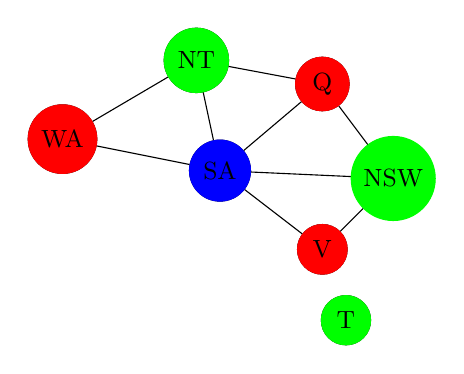
\begin{tikzpicture}[every node/.style={circle,draw}]
			\small
			\node<2> (WA) at (0, 0) {WA};
			\node<2> (NT) at (1.7, 1) {NT};
			\node<2> (SA) at (2, -0.4) {SA};
			\node<2> (Q) at (3.3, 0.7) {Q};
			\node<2> (NSW) at (4.2, -0.5) {NSQ};
			\node<2> (V) at (3.3, -1.4) {V};
			\node<2> (T) at (3.6, -2.3) {T};
			
			\draw<2-3> (SA) -- (WA) -- (NT) -- (Q) -- (NSW) -- (V);
			\draw<2-3> (SA) -- (NT);
			\draw<2-3> (SA) -- (Q);
			\draw<2-3> (SA) -- (NSW);
			\draw<2-3> (SA) -- (V);
			
			\node<3>[fill,red] at(WA) {\textcolor{black}{WA}};
			\node<3>[fill,green] at(NT) {\textcolor{black}{NT}};
			\node<3>[fill,blue] at(SA) {\textcolor{black}{SA}};
			\node<3>[fill,red] at(Q) {\textcolor{black}{Q}};
			\node<3>[fill,green] at(NSW) {\textcolor{black}{NSW}};
			\node<3>[fill,red] at(V) {\textcolor{black}{V}};
			\node<3>[fill,green] at(T) {\textcolor{black}{T}};
		\end{tikzpicture}
		\includegraphics<4 | handout:0>[width=.5\textwidth]{australia-solution}
	\end{center}
\end{frame}

\begin{frame}
	\framesubtitle{Contradição? \uncover<2->{Não...}}
	
\includegraphics[width=.45\textwidth]{Non-Counterexample_1}
	\hfill
	\includegraphics<2->[width=.45\textwidth]{Non-Counterexample_2}
\end{frame}

\begin{frame}[label=notas]
	Aplicações:
	\begin{itemize}
		\item Planejamento: tarefas conflitantes (que não podem ser realizadas ao mesmo tempo) são adjacentes.
		\vfill
		\item Alocação de Registros: recursos necessários ao mesmo tempo são adjacentes (otimização).
		\vfill
		\item Reconhecimento de padrões.
		\vfill
		\item Sudoku.
	\end{itemize}
\end{frame}%
	% %!TEX root = ED_Grafo.tex

\section{Análise de Circuitos Elétricos}
\begin{frame}[label=notas]
	A análise de circuitos elétricos com vários componentes passa pela construção
	de um sistema de equações lineares.
	\vfill
	Para análise utiliza-se: 
	\begin{itemize}
		\item as equações básicas dos componentes
		\item as leis de Kirchoff
	\end{itemize}
\end{frame}

\subsection{Leis de Kirchoff}
\begin{frame}[label=notas]
	\begin{block}{Lei das Correntes ou Leis dos Nós}
		Em um nó, a soma das correntes elétricas que entram é igual à soma das 
		correntes que saem, ou seja, um nó não acumula carga.
	\end{block}
	\begin{center}
		
\includegraphics[width=.3\textwidth]{Kirchhoff_current}\\%
		$i_1+i_4=i_2+i_3$
	\end{center}
\end{frame}

\begin{frame}[label=notas]
	\begin{block}{Lei das Tensões ou Lei das Malhas}
		A soma algébrica da diferença de potencial elétrico em um percurso 
		fechado é nula.
	\end{block}
	\begin{center}
		
\includegraphics[width=.4\textwidth]{Kirchhoff_voltage}\\%
		$v_1+v_2+v_3-v_4=0$
	\end{center}
\end{frame}

\newlength{\componentLength}\setlength{\componentLength}{15mm}%
\newlength{\wireOffset}\setlength{\wireOffset}{5mm}%
\newlength{\componentFullLength}\setlength{\componentFullLength}{\componentLength}%
\addtolength{\componentFullLength}{2\wireOffset}%
\newcommand{\componentH}[2]{%
	\draw (#2) -- ++(\wireOffset,0);
    \draw[decorate, decoration={#1}] ($(#2)+(\wireOffset,0)$) -- ++(\componentLength,0);
    \draw ($(#2)+(\wireOffset,0)+(\componentLength,0)$) -- ++(\wireOffset,0);
}%
\newcommand{\componentV}[2]{%
	\draw (#2) -- ++(0,\wireOffset);
    \draw[decorate, decoration={#1}] ($(#2)+(0,\wireOffset)$) -- ++(0,\componentLength);
    \draw ($(#2)+(0,\wireOffset)+(0,\componentLength)$) -- ++(0,\wireOffset);
}%
\newcommand{\drawCircuitCoords}{%
	\coordinate (c0) at(0,0);
	\coordinate (c1) at(0,\componentFullLength);
	\coordinate (c2) at(\componentFullLength,\componentFullLength);
	\coordinate (c3) at(2\componentFullLength,\componentFullLength);
	\coordinate (c4) at(2\componentFullLength,0);
	\coordinate (c5) at(\componentFullLength,\componentFullLength);
}%

\newcommand{\drawCircuit}[1][1-]{%
	\drawCircuitCoords%
	\uncover<#1>{
	\componentV{cell}{c0}%
    \componentH{resistor}{c1}%
    \componentH{inductor,amplitude=0.35cm, segment length=.5\componentLength}{c2}%
	\componentV{capacitor}{c4}%
    \draw (c3) -- ++(.5\componentFullLength,0);
	\componentV{resistor}{2.5\componentFullLength,0}%
    \draw (2.5\componentFullLength,0) -- (0,0);%
    }%
}%

\newcommand{\drawCircuitGraph}[1][1-]{%
	\drawCircuitCoords%
	\uncover<#1>{
    \foreach \x in {1,...,4}
		\node[draw,circle] (n\x) at(c\x) {C\x};
	\draw[->] (n1) -- (n2);
	\draw[->] (n2) -- (n3);
	\draw[->] (n3) -- (n4);
	\draw[->] (n4) -- (c0) -- (n1);
	\draw[->] (n3) -- ++(.5\componentFullLength,0) -- ++(0,-\componentFullLength) -- (n4);
	}%
}%

\begin{frame}[label=notas]
\begin{tikzpicture}[line width=1pt]
    \drawCircuit%
\end{tikzpicture}
\vfill
\begin{tikzpicture}[line width=1pt]
    \drawCircuitGraph[2]%
\end{tikzpicture}
\pause
\end{frame}
% Kirchhoff_voltage
% 
% 
% Kirchhoff's circuit laws are two equalities that deal with the conservation of charge and energy in electrical circuits, and were first described in 1845 by Gustav Kirchhoff.[1] Widely used in electrical engineering, they are also called Kirchhoff's rules or simply Kirchhoff's laws (see also Kirchhoff's laws for other meanings of that term).

% Both circuit rules can be directly derived from Maxwell's equations, but Kirchhoff preceded Maxwell and instead generalized work by Georg Ohm.%
\end{document}%
